\documentclass[12pt]{article}
%compile using XeLaTeX
\usepackage{diary_style}
\setlength{\footskip}{\paperheight
  -(0.75in+\voffset+\topmargin+\headheight+\headsep+\textheight)
  -0.75in}

%\fontspec{Times New Roman}

\DeclareMathOperator{\di}{d\!}
\newcommand*\Eval[3]{\left.#1\right\rvert_{#2}^{#3}}

\begin{document}

%\doublespacing
\vspace{1.0 \baselineskip}

\begin{flushright}
	Alexander Caines\\
	MATH-310\\
	3-29-2021\\
\end{flushright}

\begin{center}
	\textbf{\underline{EXAM 2}}
\end{center}


%\vspace{0.5 \baselineskip}

\begin{enumerate}
	\item[1.] The following are the results of running an ANOVA on the three factors (temperature, fabric denier, and air pressure) 
	at each of their respective three levels.
	\item[3.] 
		\begin{enumerate}
			\item[(a)] Below is the result of the following line of code, given the appropriate datset, $data$:
				$$model \leftarrow lm(NO3 ~ CO, data=data);\text{ } summary(model)$$ 
				\begin{figure}[!h]
					\centering
					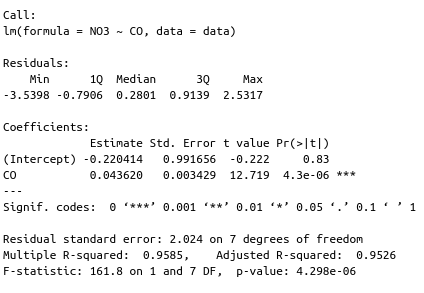
\includegraphics[width=8cm]{no3copmodel.png}
					\caption{Model of NO3 and CO data.}
				\end{figure}
			\item[(****b)] The equation produced by the linear regression in R was 
$$\hat{y} = 13.63x + 21.97 $$ So, the prediction for
 $x=400$ is $5473.97$. Given that the mean of CO is $211.89$, the following work shows 
		that the prediction interval is $(-139.5264, 563)$.
			$$yhat = mean(data$CO);\text{ }t = 0.627;\text{ };error = 21.734;\text{ }r^2 = deviance(model)$$
			$$bound = t_int*sqrt(error_int*(1/length(data)+1+r2))
$$		
			Since the predicted value lies outside of the prediction interavl, the linear regression 
			could not have accurately predicted it.
			\item[(c)] Without the largest value of CO, the fitted equation is $\hat{y} = 15.21x + 21.70$. Yielding $6105.7$ as 
			the prediction: a number far outside the previous prediction interval. So the largest CO value has a substantial 
			effect on the model.
		\end{enumerate}
	\item[4.] Below I show that $SSE = S_{yy} - \hat{\beta}_1S_{xy}$.
		\begin{center}
		\begin{math}
		\begin{aligned}
			SSE &= \sum{y^2_i} - \hat{\beta}_0\sum{y_i} - \hat{\beta}_1\sum{x_iy_i}\\
			&= \sum{y^2_i} - (\bar{y} - \hat{\beta}_1\bar{x})\sum{y_i} - \hat{\beta}_1\sum{x_iy_i}\\
			&= \sum{y^2_i} -\bar{y}\sum{y_i} + \hat{\beta}_1\bar{x}\sum{y_i} - \hat{\beta}_1\sum{x_iy_i}\\
			&= \sum{y^2_i} -\frac{1}{n}\sum{y_i}\sum{y_i} + \hat{\beta}_1(\sum\bar{x}{y_i} - \sum{x_iy_i})\\
			&= \sum{y^2_i} -\frac{1}{n}(\sum{y_i})^2 - \hat{\beta}_1((\sum{x_iy_i}) - \sum{\bar{x}y_i})\\
			&= S_{yy} - \hat{\beta}_1((\sum{x_iy_i}) - \sum{\bar{x}y_i})\\
			&= S_{yy} - \hat{\beta}_1S_{xy}\\
		\end{aligned}
		\end{math}
		\end{center}

\end{enumerate}

\end{document}
